\documentclass{article}
\usepackage{amsmath,epsfig,rotating}
\usepackage{subcaption} % For aligning subfigures
\usepackage{pdfpages}

\begin{document}

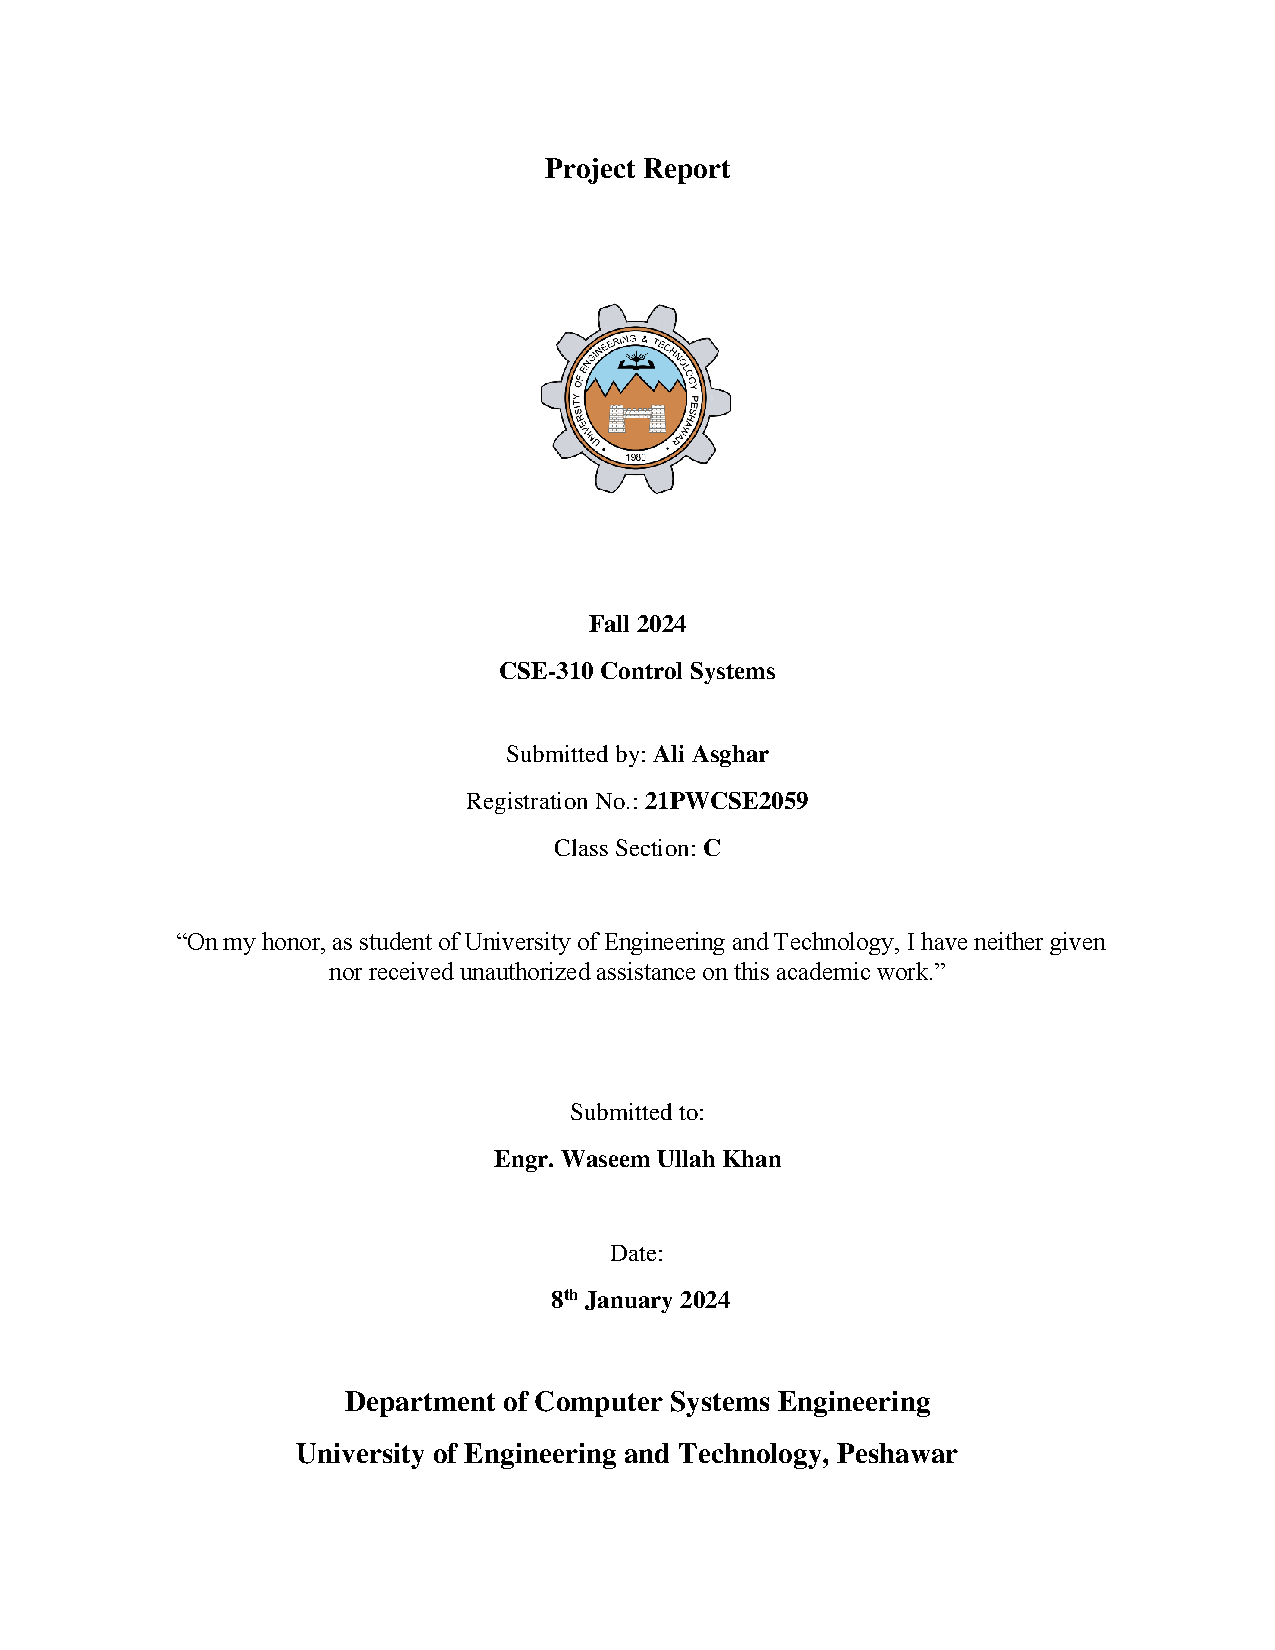
\includepdf[pages={1}]{CoverPage.pdf}  % Include pages 1 to 3

\begin{flushleft}
%{\sc \Large Control Systems - Project Report} \hfill \\ $ $ \\
%\medskip
%Name: Ali Asghar \\
%Enrollment Number: 21PWCSE2059\\
%Section: C \\
%\today
\end{flushleft}

\tableofcontents
\newpage

\section{Problem which is considered}
\noindent Perform the following for Problem 22 at Page 148:\\
%a. Obtain state-space representation for the system (without obtaining any transfer function). \\
%b. Choose the output matrix as you like (except identity matrix - and make the system observable). \\
%c. Check the stability of the system using all methods that you know.\\
%d. Compute the controllability and observability for the system. If the system is controllable, place the controller poles at (-3, -5) and observer poles at a location which is faster than the controller poles.\\
%e. Simulate the system using observer based feedback controller and show all the responses.
a. Consider the state-space of Problem 22, Page 148 of Norman Nise Book Edition 5. \\
b. Check the stability of the system using all the methods that you know. \\
c. Compute the controllability and observability for the system. If the system is unstable, design a suitable controller for it. \\
d. Simulate the system using the controller that you design and show all the responses.\\
e. Design a PID Controller and show the response of the system using PID Controller. Compare the results obtained in part d and e.\\
f. Compute the steady state errors before and after designing controller.\\

The Problem 22 at Page 148 is qouted as:
"`
In the past, Type-1 diabetes patients had to inject themselves with insulin three to four times a day.
New delayed-action insulin analogues such as insulin Glargine require a single daily dose. A similar procedure to
the one described in the Pharmaceutical Drug Absorption case study of this chapter is used to find a model for
the concentration-time evolution of plasma for insulin Glargine. For a specific patient, state-space model matrices
are given by (Tarín, 2007)"'
\vskip10pt
\[
A = \begin{bmatrix}
-0.435 & 0.209 & 0.02\\
0.268 & -0.394 & 0\\
0.227 & 0 & -0.02\end{bmatrix}
%\]
%\[
B = \begin{bmatrix}
1 \\
0 \\
0 
\end{bmatrix}
\]
%\vskip10pt

\[
C=\begin{bmatrix}
0.003 & 0 & 0
\end{bmatrix}
D = 0
\]
where the state vector is given by

\[
x = \begin{bmatrix}
x_1 \\
x_2 \\
x_3
\end{bmatrix}
\]

The state variables are:
\begin{itemize}
    \item \(x_1\): insulin amount in the plasma compartment,
    \item \(x_2\): insulin amount in the liver compartment,
    \item \(x_3\): insulin amount in the interstitial (body tissue) compartment.
\end{itemize}

The system input is \(u\): external insulin flow.

The system output is \(y\): plasma insulin concentration.
\vskip30pt

\section{Solution}
In this report, we address the the above problem and explain each subproblem in detail.

\subsection{State-space Representation of the System}
The state-space representation of the system can be written as follows:
\begin{equation}
\begin{bmatrix} \dot{x_1}\\  \dot{x_2}\\ \dot{x_3} \end{bmatrix}
= \begin{bmatrix}
-0.435 & 0.209 & 0.02\\
0.268 & -0.394 & 0\\
0.227 & 0 & -0.02\end{bmatrix}
\begin{bmatrix} x_1\\  x_2 \\ x_3 \end{bmatrix} +
\begin{bmatrix}
1 \\
0 \\
0 \end{bmatrix}
u(t)
%\begin{bmatrix} u_1 \end{bmatrix}
\end{equation}

\begin{equation}
y=\begin{bmatrix}
0.003 & 0 & 0
\end{bmatrix}x
\end{equation}

%If the state-space for your problem is not obtained, obtain it. Mention the state-space here in this section.


\subsection{Stability analysis of the system}
In this section, we analyze the stability of the system. The stability can be checked using different ways namely eigen values, step response, poles, root locus and RH-stability criteria. 

\subsubsection{Eigen Values}
For our case, the system is of 3rd order and therefore there will be three eigen values. Let $\lambda_1$ , $\lambda_2$ and $\lambda_3$ denote the eigen values of the system. The values of eigen values can be written as follows:
\begin{equation} \lambda_1 = -0.6560,  \lambda_2 = -0.1889, \lambda_3 = -0.0042 \end{equation}
   
	
As we can see all of the eigen values are negative, which indicates the system is stable.

\subsubsection{Poles}
Next, we verify the same fact by observing the poles of the system. Let $p_1$, $p_2$ and $p_3$ denote the poles of the system. The values for poles are as follows:
\begin{equation} p_1 = -0.6560,  p_2 = -0.1889, p_3 = -0.0042 \end{equation}


We observe here again that all of the poles are positive, which indicates the system is stable. 

\subsubsection{Step Response}
Next, we verify the same fact by seeing the step-response of the system. The step-response of open-loop system is shown in Figure \ref{fig:stepResponse}.

\begin{figure}[h!]
	\centering
	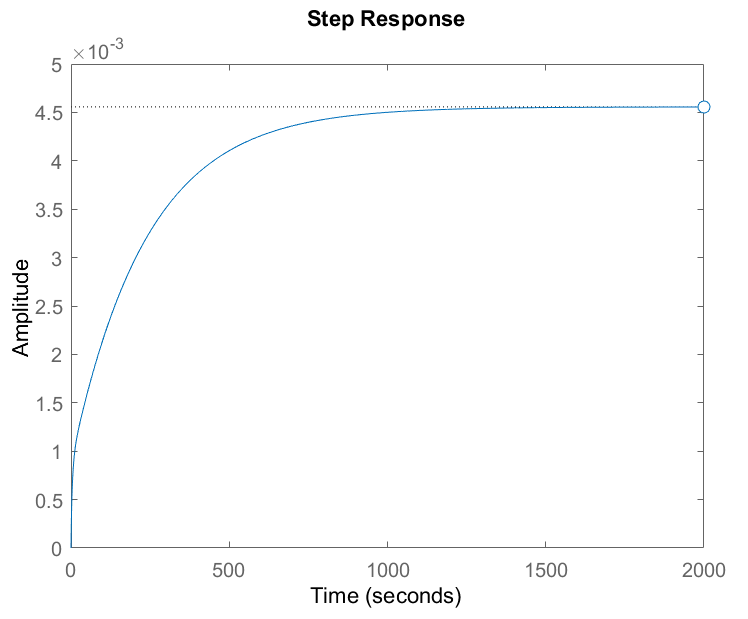
\includegraphics[scale=0.75]{images/stepResponse.png}
	\caption{Plot of step response in MATLAB.}
	\label{fig:stepResponse}
\end{figure}

\begin{figure}[h!]
	\centering
	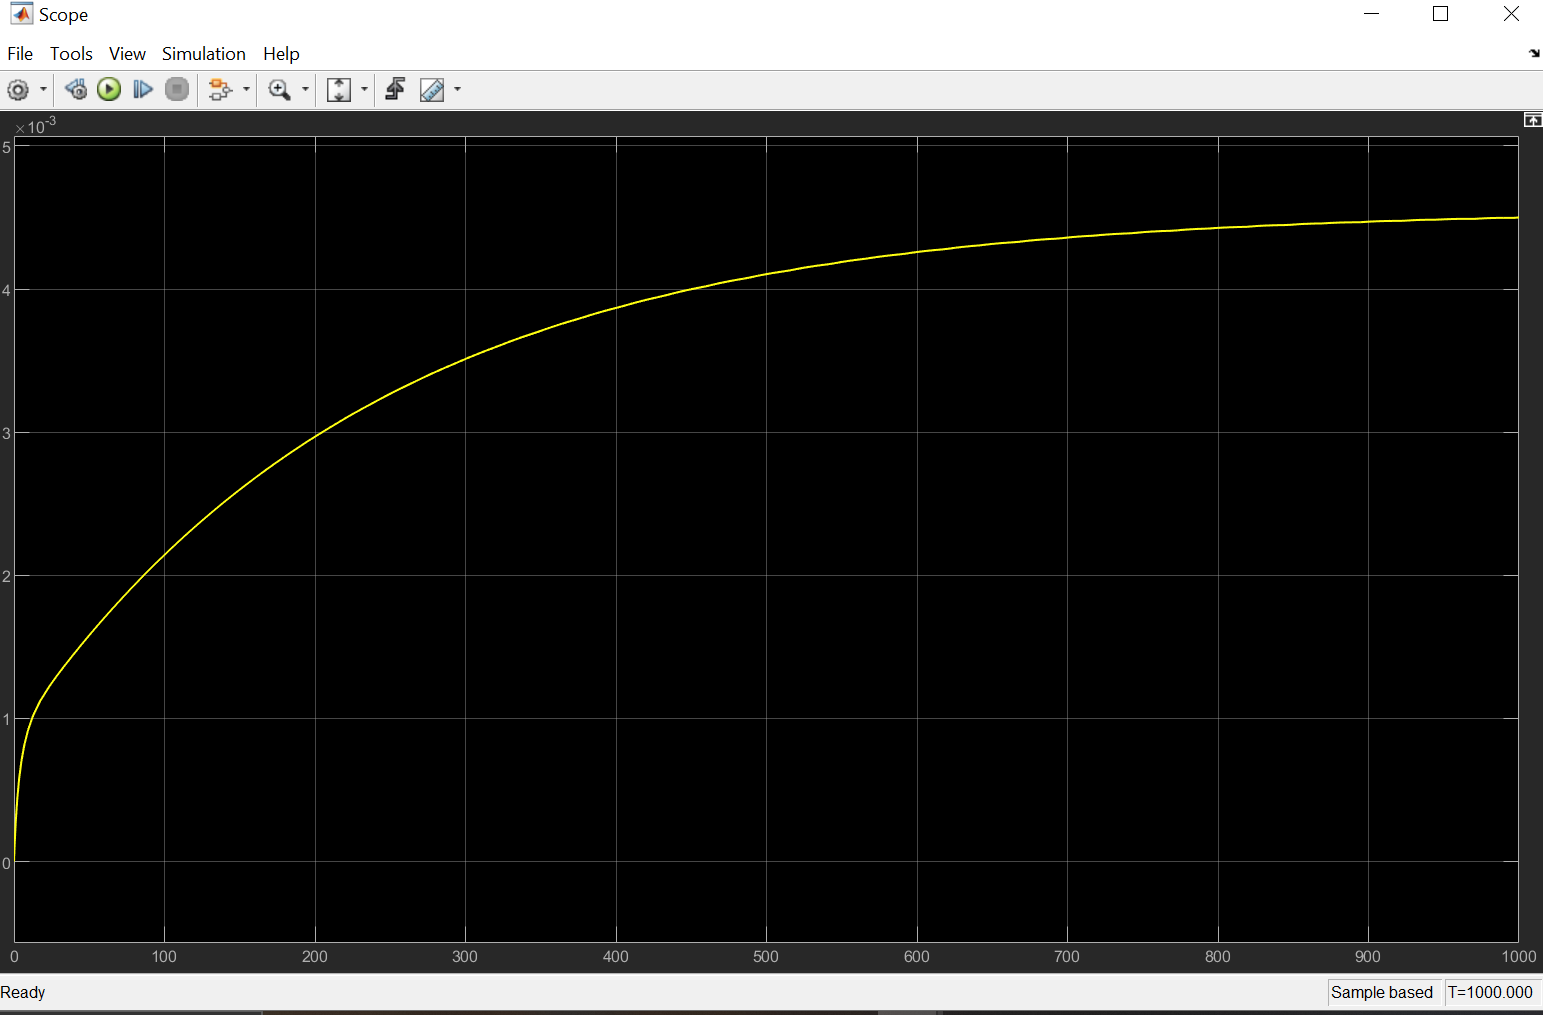
\includegraphics[scale=0.5]{images/stepResponse_Simulink.png}
	\caption{Plot of step response in Simulink.}
	\label{fig:stepResponse}
\end{figure}

From Figure \ref{fig:stepResponse}, we can do the following analysis: \\
\begin{equation}\begin{aligned}
\%OS & = 0\%\\
T_r & = 496s\\
T_s & = 882s\\
Peak Value & = 0.00456\\
Final Value & = 0.00456 \end{aligned} \notag \end{equation}

%\subsubsection{Routh-Hurwitz Criteria}
%\noindent Next, we construct a Routh-Hurwitz table to check the stability of the system.
%The transfer function of the system is:
%\[
%H(s) = \frac{0.0003 s^2 + 0.0001242 s + 2.364\times10^{-6}}{s^3 + 0.849 s^2 + 0.1274 s + 0.0005188}
%\]

%\begin{table}[!h] \begin{center}
%\begin{tabular}{|l|c|l|} \hline
%$s^3$  & 1 & 0.1274 \\ \hline
%$s^2$  & 0.849 & 0.0005188 \\ \hline
%$s^1$  & $-\frac{1}{0.849}\times\begin{vmatrix} 1 & 0.1274\\ 0.849 & 0.0005188 \end{vmatrix}=0.126$ & $-\frac{1}{0.849}%\times\begin{vmatrix} 1 & 0\\ 0.849 & 0 \end{vmatrix}=0$ \\

%$s^0$  & $-\frac{1}{0.126}\times\begin{vmatrix} 0.849 & 0.0005188\\ 0.126 & 0 \end{vmatrix}=0.0005188$ & $-\frac{1}{0.126}\times\begin{vmatrix} 0.849 & 0\\ 0.126 & 0 \end{vmatrix}=0$ 

%\\ \hline
%\end{tabular} \end{center}
%\end{table}

\noindent As there are no sign changes in the first column, the system is stable.

\subsubsection{Pole-Zero Map}
Next, I plotted the system's pole-zero map to analyze stability. All poles are in the left-half plane, as shown in Figure \ref{fig:poleZeroMap}. This confirms the system is stable.

\begin{figure}[h!]
	\centering
	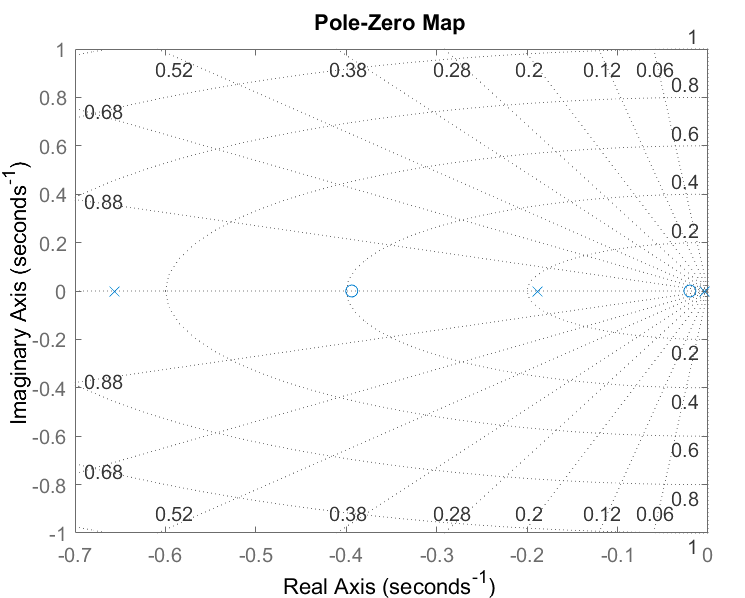
\includegraphics[scale=0.75]{images/poleZeroMap.png}
	\caption{Pole Zero Map of the System}
	\label{fig:poleZeroMap}
\end{figure}


\subsubsection{Root Locus} 
I performed a root locus analysis to observe pole movement as the gain K changes. Figure \ref{fig:rootLocus} shows all poles stay in the left-half plane, verifying the system's stability.

\begin{figure}[h!]
	\centering
	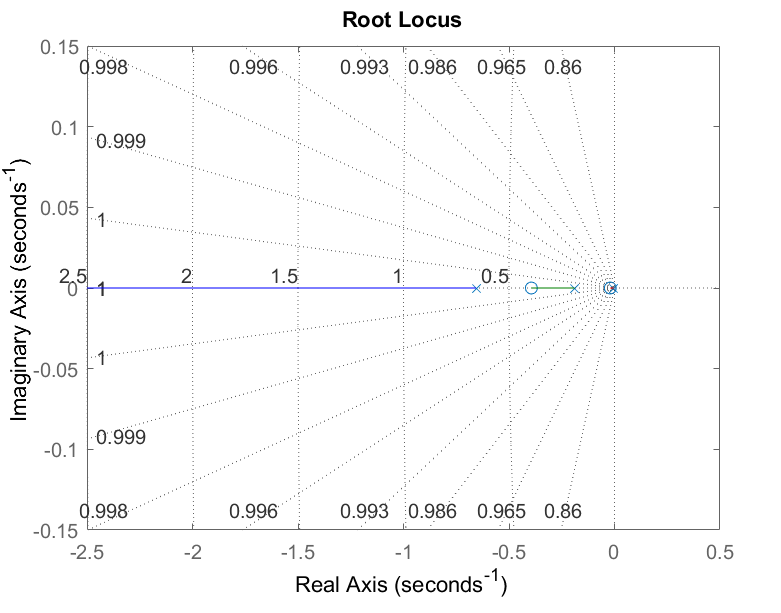
\includegraphics[scale=0.75]{images/rootLocus.png}
	\caption{Root Locus Plot of System.}
	\label{fig:rootLocus}
\end{figure}


\subsection{Controllability analysis of the system}
As the system is stable, there's no need for controllability analysis.

\subsection{Observability analysis of the system}
As the system is stable, there's no need for observability analysis.

\subsection{Controller Design for the system}
As the system is stable, there's no need to design Full-State Feedback Controller or Observer-based Controller.
However, to reduce the steady-state error, we can design a PID Controller for it.

%\subsubsection{Basic Theory}
%The following sections explain the basic concepts and equations for PID Controller design.

\subsubsection{Steady-State Error}

The steady-state error (SSE) is an important measure of a control system’s performance, indicating how accurately the system tracks the reference input in the steady state.

For this system in a unity feedback configuration, the steady-state error depends on the system type and the input signal. Using the \textit{Final Value Theorem}, the steady-state error is calculated as:
\[
\text{SSE} = \lim_{s \to 0} s \cdot E(s)
\]
where \( E(s) \) is the Laplace transform of the error signal, \( E(s) = R(s) - T(s) \cdot R(s) \). For a unity feedback system, \( E(s) = \frac{R(s)}{1 + G(s)} \), where \( G(s) \) is the open-loop transfer function.

\paragraph{Step Input (\( R(s) = \frac{1}{s} \))}  
For a step input, the steady-state error is given by:
\[
\text{SSE} = \frac{1}{1 + K_p}
\]
where \( K_p = \lim_{s \to 0} G(s) \) is the \textit{position error constant}. %If the system is \textit{Type 1} or higher (contains at least one pole at the origin), the steady-state error for a step input is zero.

\paragraph{Ramp Input (\( R(s) = \frac{1}{s^2} \))}  
For a ramp input, the steady-state error is given by:
\[
\text{SSE} = \frac{1}{K_v}
\]
where \( K_v = \lim_{s \to 0} s \cdot G(s) \) is the \textit{velocity error constant}. %For a \textit{Type 0} system, \( K_v \) is finite, resulting in a nonzero SSE. For a \textit{Type 1} or higher system, the SSE for ramp input is zero.

\paragraph{Parabolic Input (\( R(s) = \frac{1}{s^3} \))}  
For a parabolic input, the steady-state error is:
\[
\text{SSE} = \frac{1}{K_a}
\]
where \( K_a = \lim_{s \to 0} s^2 \cdot G(s) \) is the \textit{acceleration error constant}. %Only a \textit{Type 2} or higher system can achieve zero SSE for a parabolic input.

---

\subsubsection{PID Controller Design}

To reduce the steady-state error, we design a PID controller for the system. The transfer function of a PID controller is:
\[
C(s) = K_p + \frac{K_i}{s} + K_d \cdot s
\]
where:
\begin{itemize}
    \item \( K_p \) is the proportional gain, which reduces the rise time and improves the transient response.
    \item \( K_i \) is the integral gain, which eliminates the steady-state error by adding a pole at the origin.
    \item \( K_d \) is the derivative gain, which improves system stability and reduces overshoot.
\end{itemize}

The overall closed-loop transfer function with the PID controller becomes:
\[
T(s) = \frac{C(s)G(s)}{1 + C(s)G(s)}
\]

\subsection{Controller Design for given System}
%\subsubsection{Response to Input Signals}

To analyze the steady-state error for different types of input signals, we apply the \textit{Final Value Theorem}, which states:
\[
\text{SSE} = \lim_{s \to 0} s \cdot E(s)
\]
where \(E(s)\) is the Laplace transform of the error signal. For a unity feedback system, \(E(s) = \frac{R(s)}{1 + G(s)}\), and \(G(s)\) is the open-loop transfer function.

Given the system:
\[
G(s) = \frac{0.0003 s^2 + 0.0001242 s + 2.364 \times 10^{-6}}{s^3 + 0.849 s^2 + 0.1274 s + 0.0005188}
\]
we calculate the steady-state error for different input types.


\subsubsection{Step Input (\( R(s) = \frac{1}{s} \))}
\label{PIDControllerDesignStep}
For a step input, the steady-state error is given by:
\[
\text{SSE} = \lim_{s \to 0} s \cdot \frac{\frac{1}{s}}{1 + G(s)} = \frac{1}{1 + K_p}
\]
where \( K_p = \lim_{s \to 0} G(s) \) is the \textit{position error constant}.

For the given system:
\[
G(s) \big|_{s = 0} = \frac{2.364 \times 10^{-6}}{0.0005188} \approx 0.00456
\]

Thus:
\[
\text{SSE} = \frac{1}{1 + 0.00456} \approx 0.9955
\]


\subsubsection{Ramp Input (\( R(s) = \frac{1}{s^2} \))}

For a ramp input, the steady-state error is given by:
\[
\text{SSE} = \lim_{s \to 0} s \cdot \frac{\frac{1}{s^2}}{1 + G(s)} = \frac{1}{K_v}
\]
where \( K_v = \lim_{s \to 0} s \cdot G(s) \) is the \textit{velocity error constant}.

For the given system:
\[
K_v = \lim_{s \to 0} s \cdot \frac{0.0003 s^2 + 0.0001242 s + 2.364 \times 10^{-6}}{s^3 + 0.849 s^2 + 0.1274 s + 0.0005188} = 0
\]

Thus:
\[
\text{SSE} = \frac{1}{0} = \infty
\]



\subsubsection{Parabolic Input (\( R(s) = \frac{1}{s^3} \))}

For a parabolic input, the steady-state error is given by:
\[
\text{SSE} = \lim_{s \to 0} s \cdot \frac{\frac{1}{s^3}}{1 + G(s)} = \frac{1}{K_a}
\]
where \( K_a = \lim_{s \to 0} s^2 \cdot G(s) \) is the \textit{acceleration error constant}.

For the given system:
\[
K_a = \lim_{s \to 0} s^2 \cdot \frac{0.0003 s^2 + 0.0001242 s + 2.364 \times 10^{-6}}{s^3 + 0.849 s^2 + 0.1274 s + 0.0005188} = 0
\]

Thus:
\[
\text{SSE} = \frac{1}{0} = \infty
\]

\section{MATLAB Code}
\begin{figure}[h!]
	\centering
	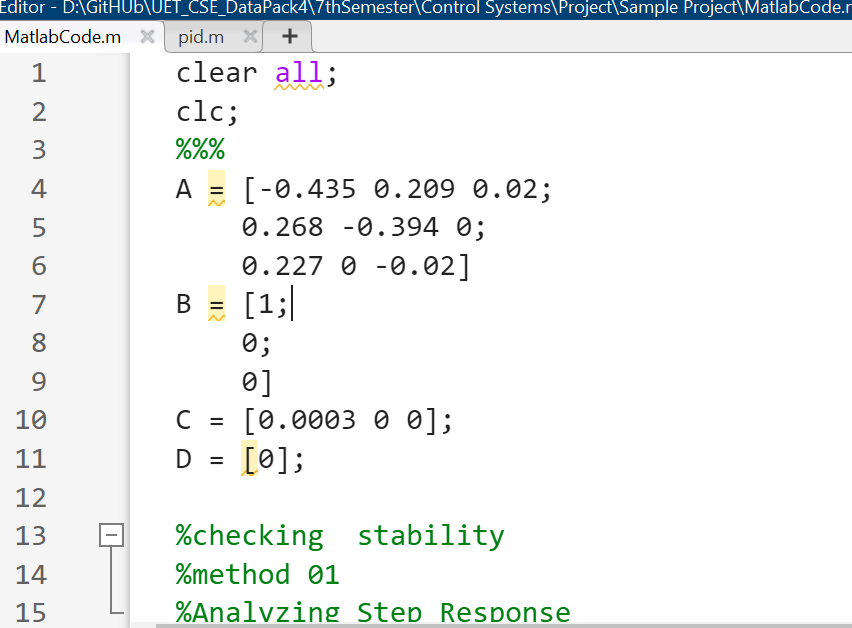
\includegraphics[scale=0.85]{images/MatlabCode1.png}
	\caption{MATLAB Code Part 1}
	\label{fig:MatlabCode2}
\end{figure}

\begin{figure}[h!]
	\centering
	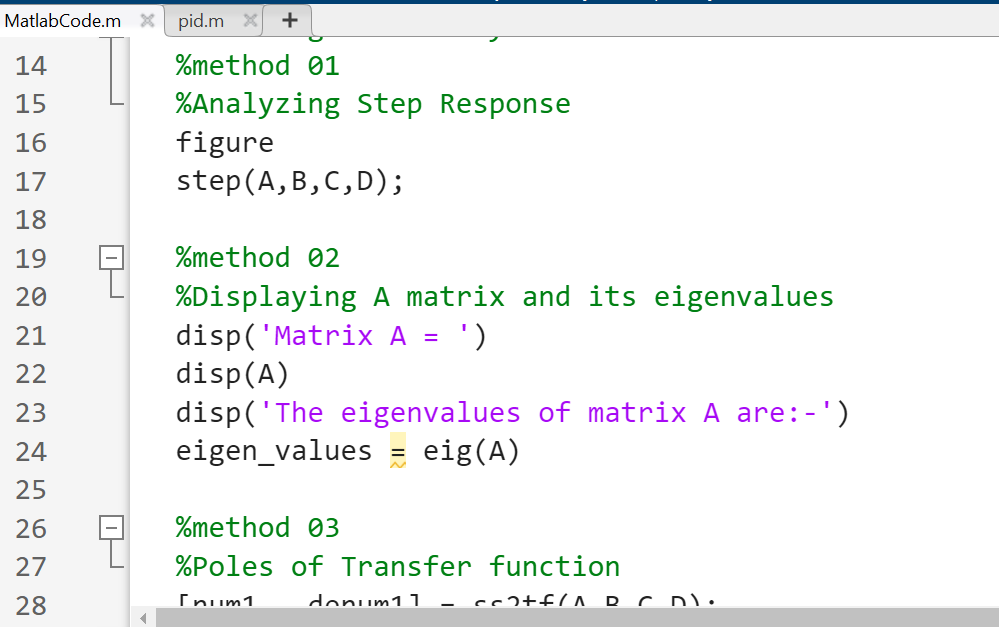
\includegraphics[scale=0.75]{images/MatlabCode2.png}
	\caption{MATLAB Code Part 2}
	\label{fig:MatlabCode2}
\end{figure}

\begin{figure}[h!]
	\centering
	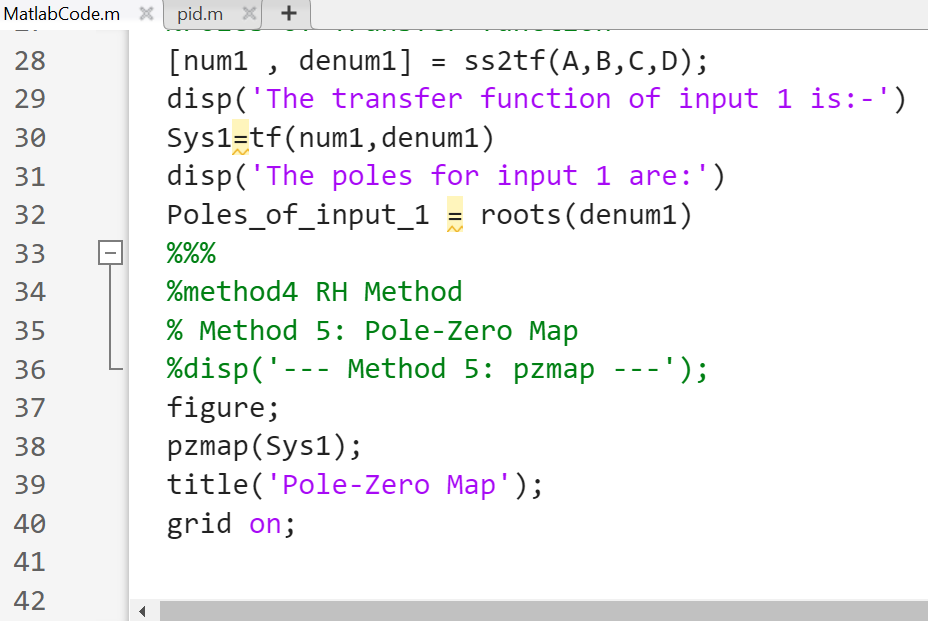
\includegraphics[scale=0.75]{images/MatlabCode3.png}
	\caption{MATLAB Code Part 3}
	\label{fig:MatlabCode3}
\end{figure}

\begin{figure}[h!]
	\centering
	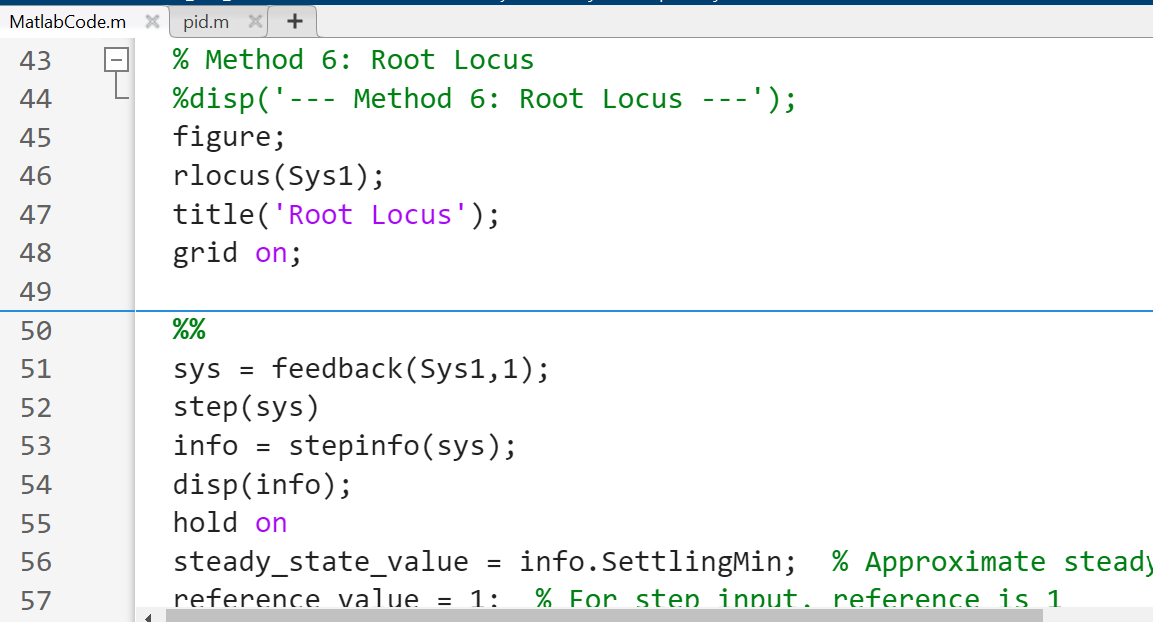
\includegraphics[scale=0.75]{images/MatlabCode4.png}
	\caption{MATLAB Code Part 2}
	\label{fig:MatlabCode4}
\end{figure}

\begin{figure}[h!]
	\centering
	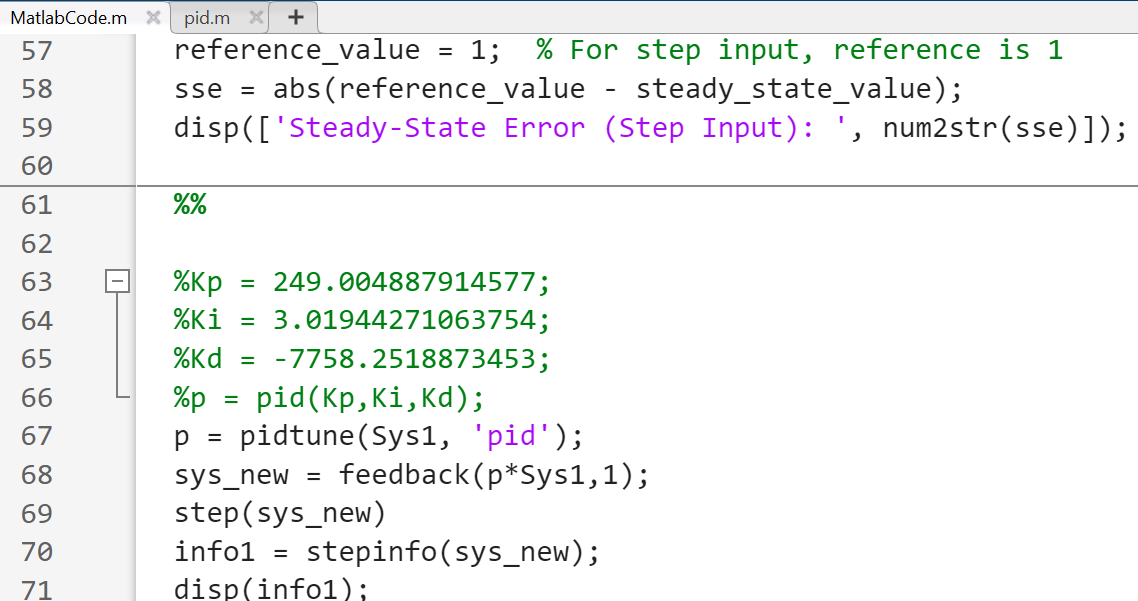
\includegraphics[scale=0.75]{images/MatlabCode5.png}
	\caption{MATLAB Code Part 5}
	\label{fig:MatlabCode5}
\end{figure}

\begin{figure}[h!]
	\centering
	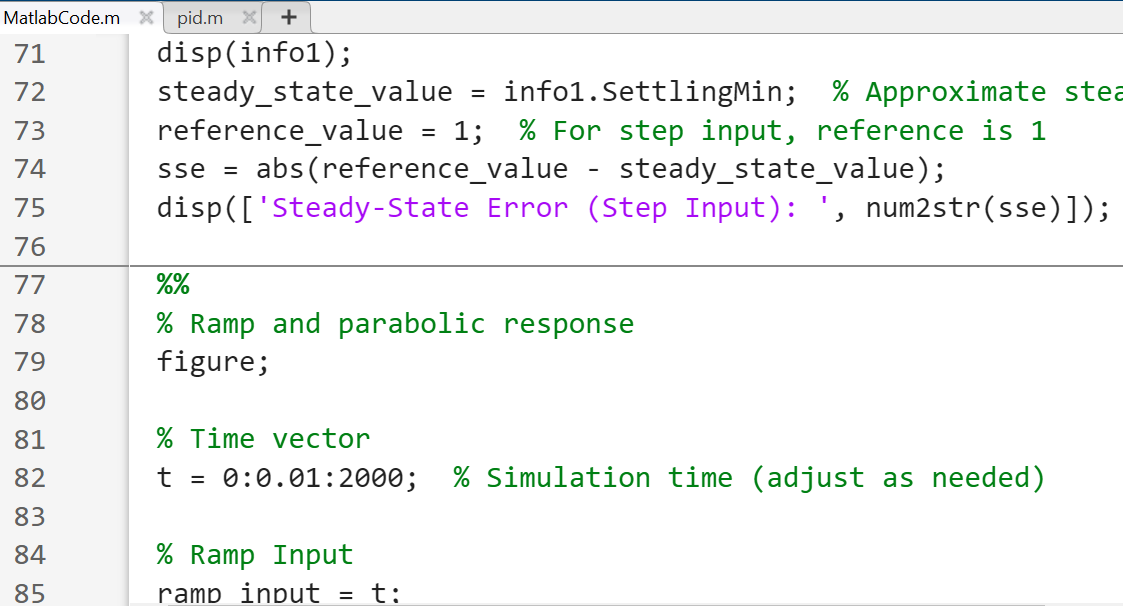
\includegraphics[scale=0.75]{images/MatlabCode6.png}
	\caption{MATLAB Code Part 6}
	\label{fig:MatlabCode4}
\end{figure}

\begin{figure}[h!]
	\centering
	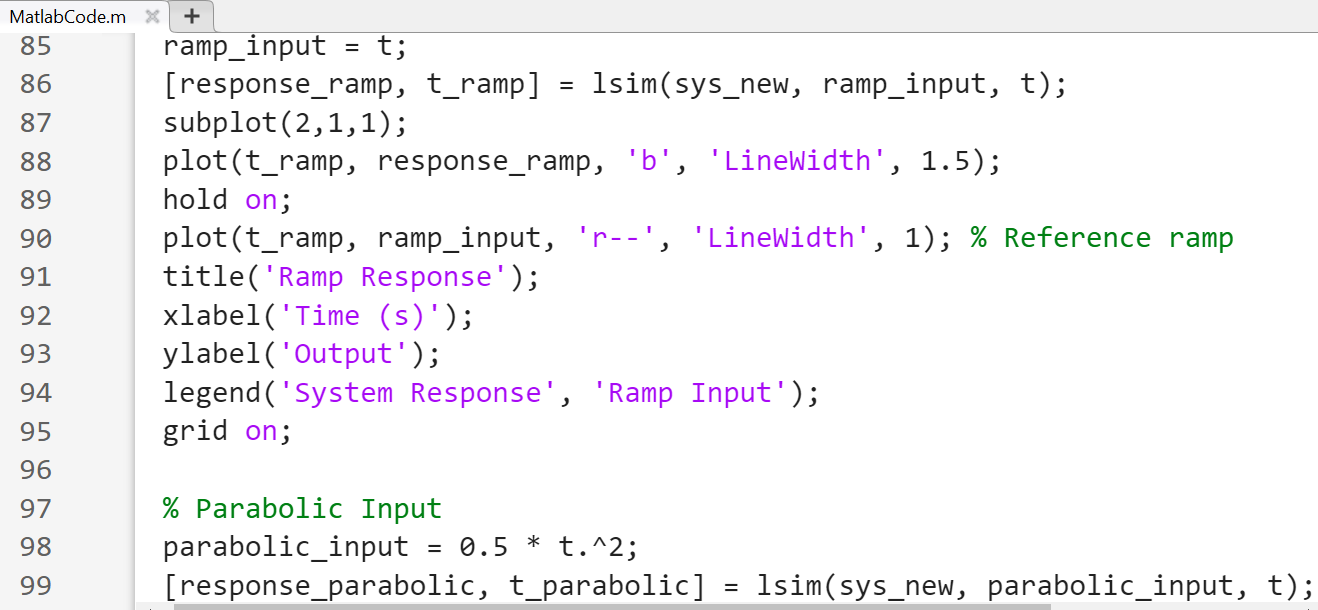
\includegraphics[scale=0.65]{images/MatlabCode7.png}
	\caption{MATLAB Code Part 7}
	\label{fig:MatlabCode5}
\end{figure}

\begin{figure}[h!]
	\centering
	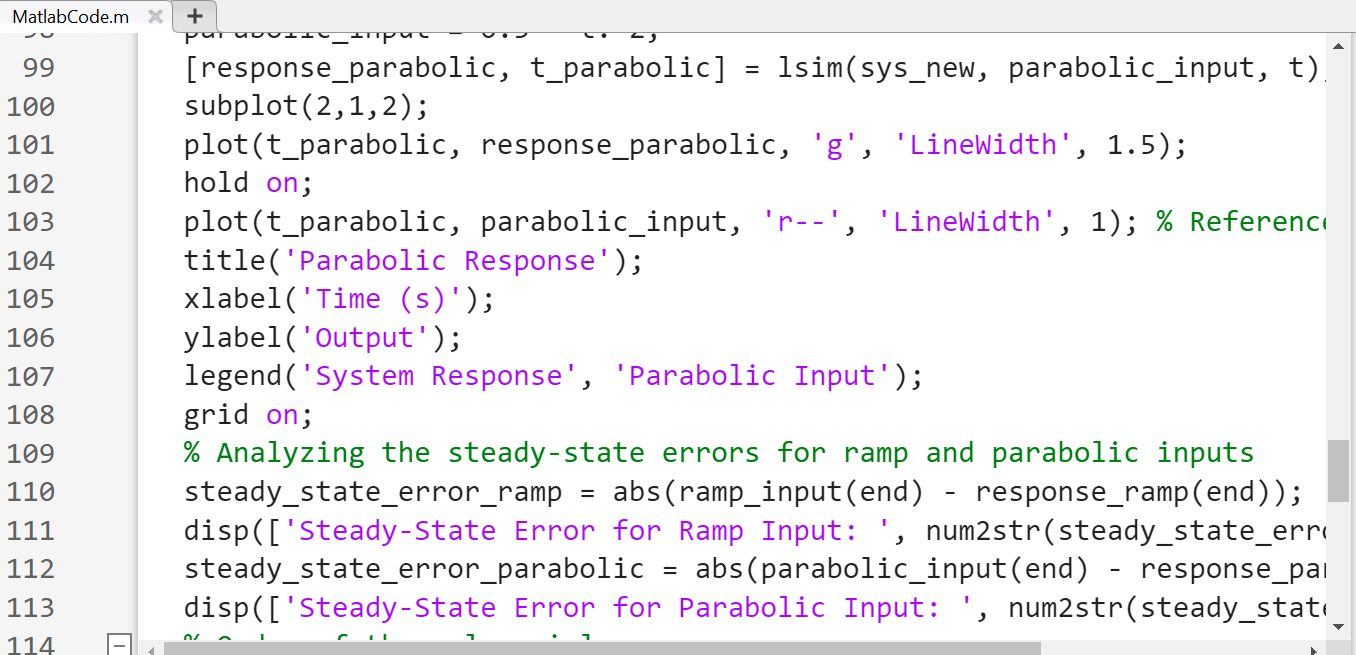
\includegraphics[scale=0.65]{images/MatlabCode8.png}
	\caption{MATLAB Code Part 8}
	\label{fig:MatlabCode5}
\end{figure}


\section{Results and Discussions}
We simulated the above system. The schematic for simulation (using Simulink) is shown in Figure \ref{fig:PIDController} and the values for Kp, Ki, Kd are shown in Figure \ref{fig:PIDController}.

\begin{figure}[h!]
	\centering
	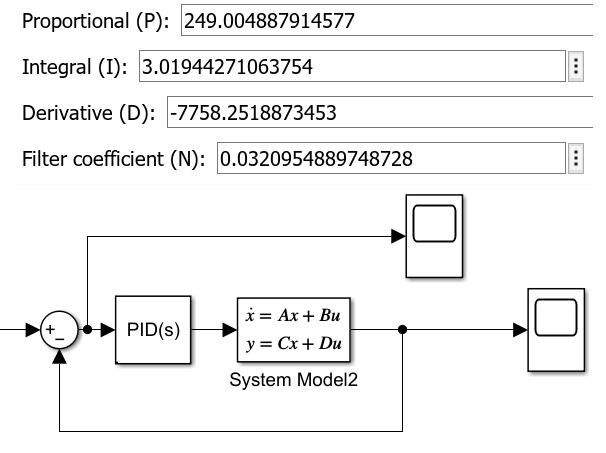
\includegraphics[scale=0.75]{images/PIDController.png}
	\caption{PID Controller in Simulink}
	\label{fig:PIDController}
\end{figure}


\subsection{SSE for Step Response}
\label{SSE_StepResponseSec}
This section describes the SSE computation before and after PID Design using Step Signal as input.


\subsubsection{SSE Calculation before PID Design}
The steady-state error was calculated by making a unity closed loop system. The sketch can be seen in the figure \ref{fig:SSE_Sketch}. The value of SSE is same as calculated in \ref{PIDControllerDesignStep}

\begin{figure}[h!]
	\centering
	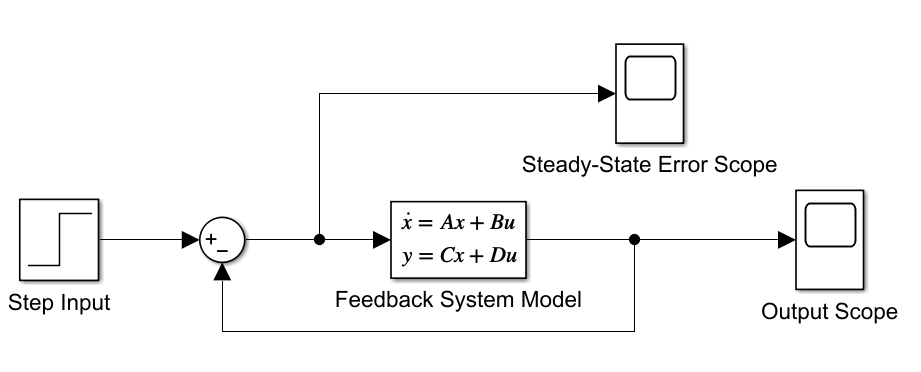
\includegraphics[scale=0.75]{images/SSE_Sketch.png}
	\caption{Unity Feedback System With Step as Input}
	\label{fig:SSE_Sketch}
\end{figure}

\begin{figure}[h!]
	\centering
	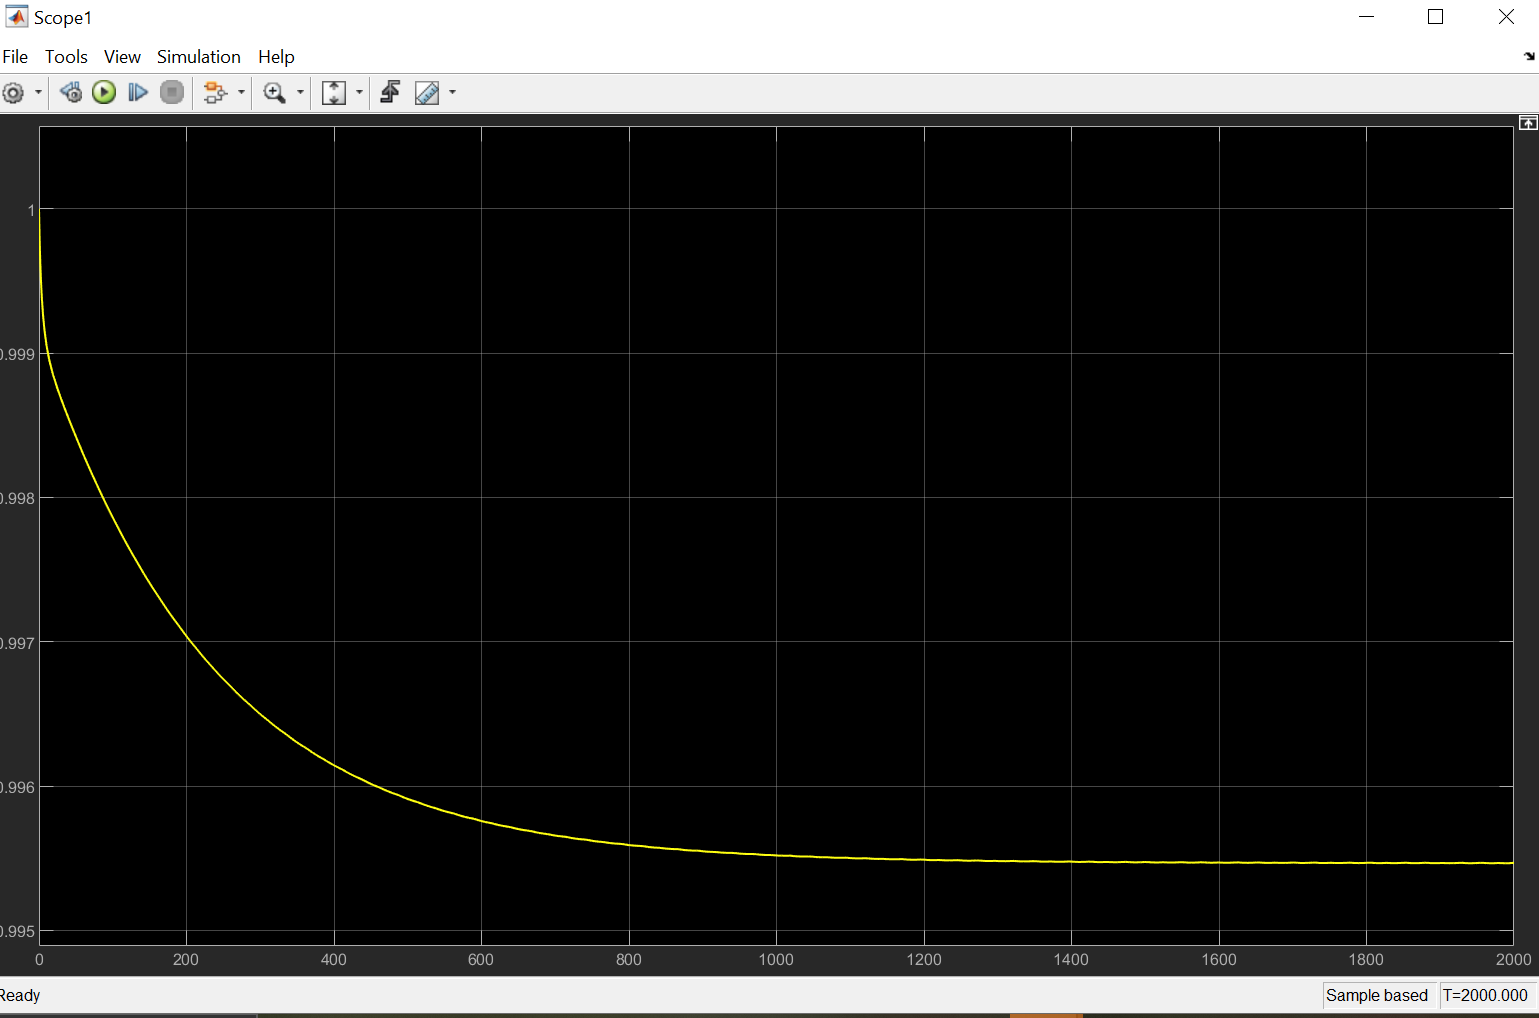
\includegraphics[scale=0.5]{images/SSE_BeforePID_Simulink.png}
	\caption{SSE Calculation before PID in Simulink}
	\label{fig:SSE_BeforePID_Simulink}
\end{figure}



\subsubsection{SSE Calculation after PID Design}
After connecting the PID Controller in series as shown in Figure \ref{fig:PIDController}, the SSE reaches almost to zero and we get a stable response at 1. The step response is shown in figure \ref{fig:stepResponse_PID_MATLAB} (MATLAB) and Figure \ref{fig:stepResponse_PID_Simulink} (Simulink). The SSE values can be verified from Figure \ref{fig:SSE_AfterPID_Simulink} (Simulink). A comparison of before and after SSE can also be seen in Figure \ref{fig:SSE_MATLAB}.


\begin{figure}[h!]
	\centering
	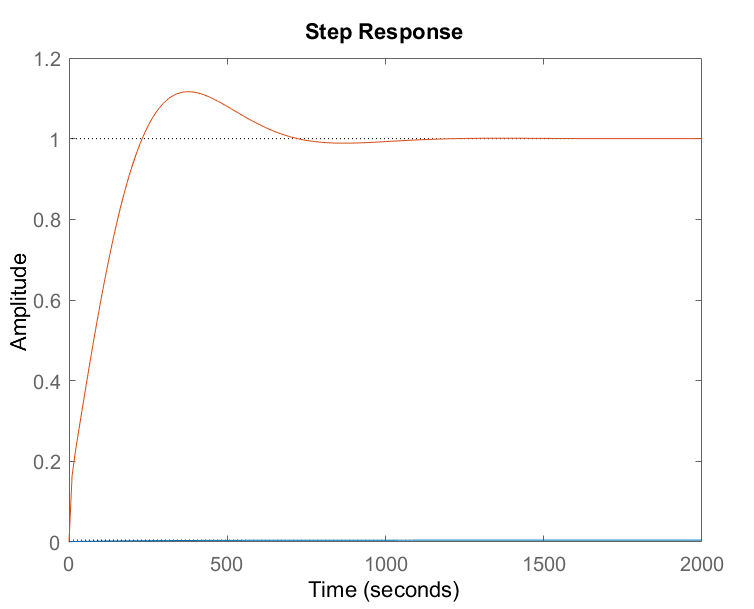
\includegraphics[scale=0.75]{images/stepResponse_PID_MATLAB.png}
	\caption{Step Response after PID in MATLAB}
	\label{fig:stepResponse_PID_MATLAB}
\end{figure}

\begin{figure}[h!]
	\centering
	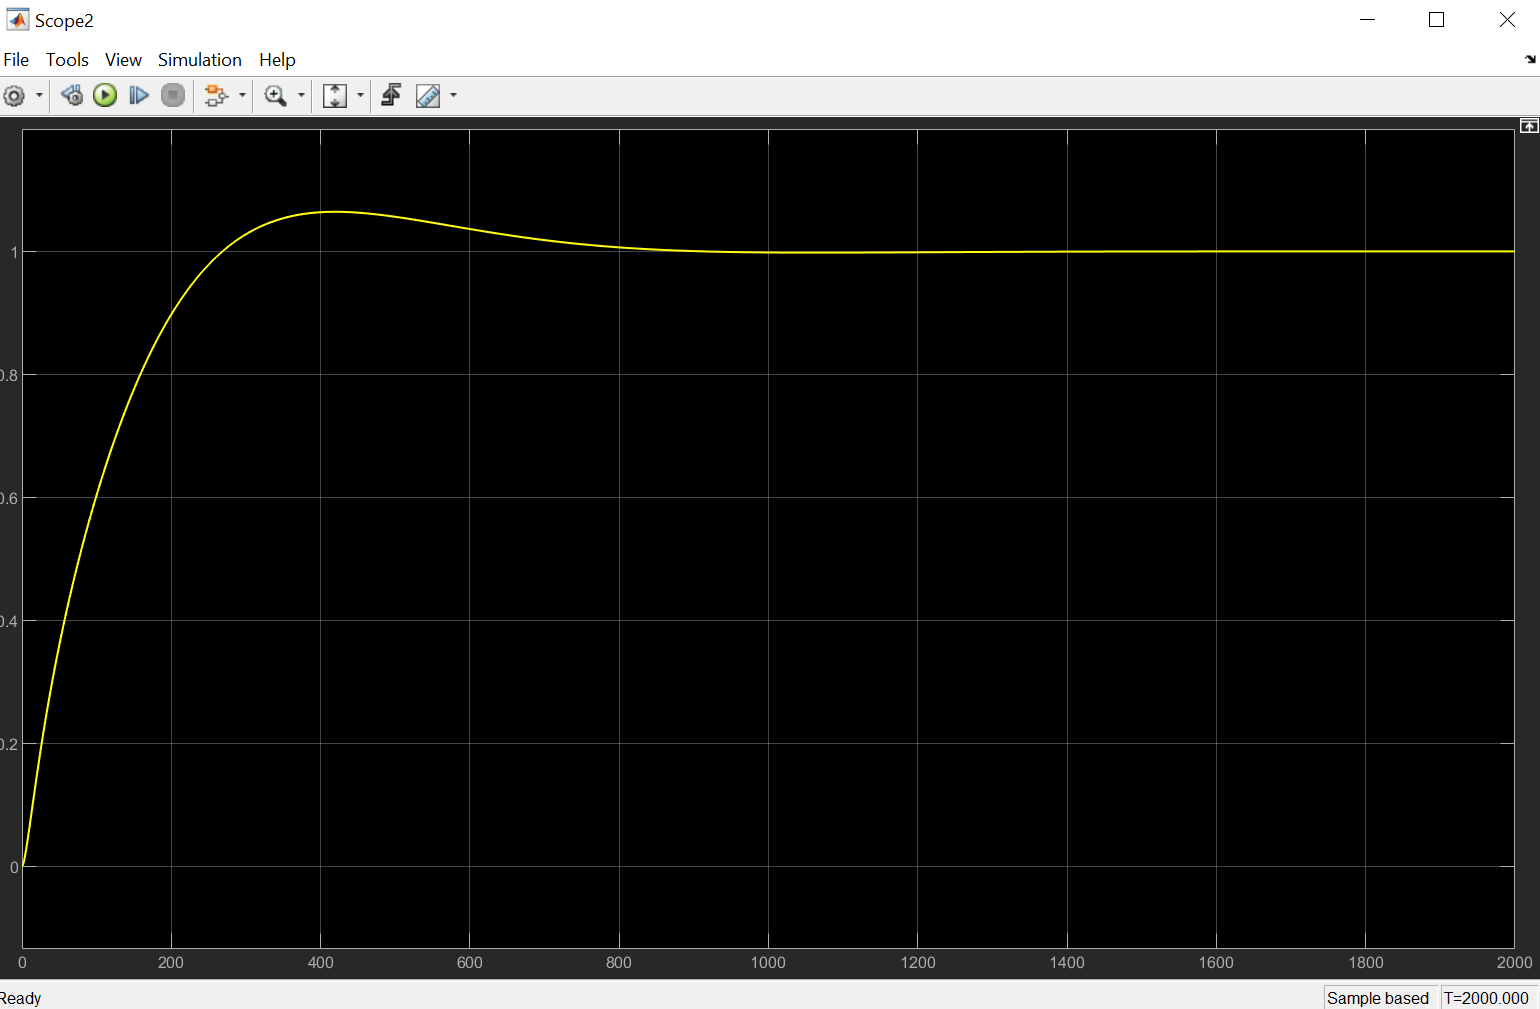
\includegraphics[scale=0.45]{images/stepResponse_PID_Simulink.png}
	\caption{Step Response after PID in Simulink}
	\label{fig:stepResponse_PID_Simulink}
\end{figure}

\begin{figure}[h!]
	\centering
	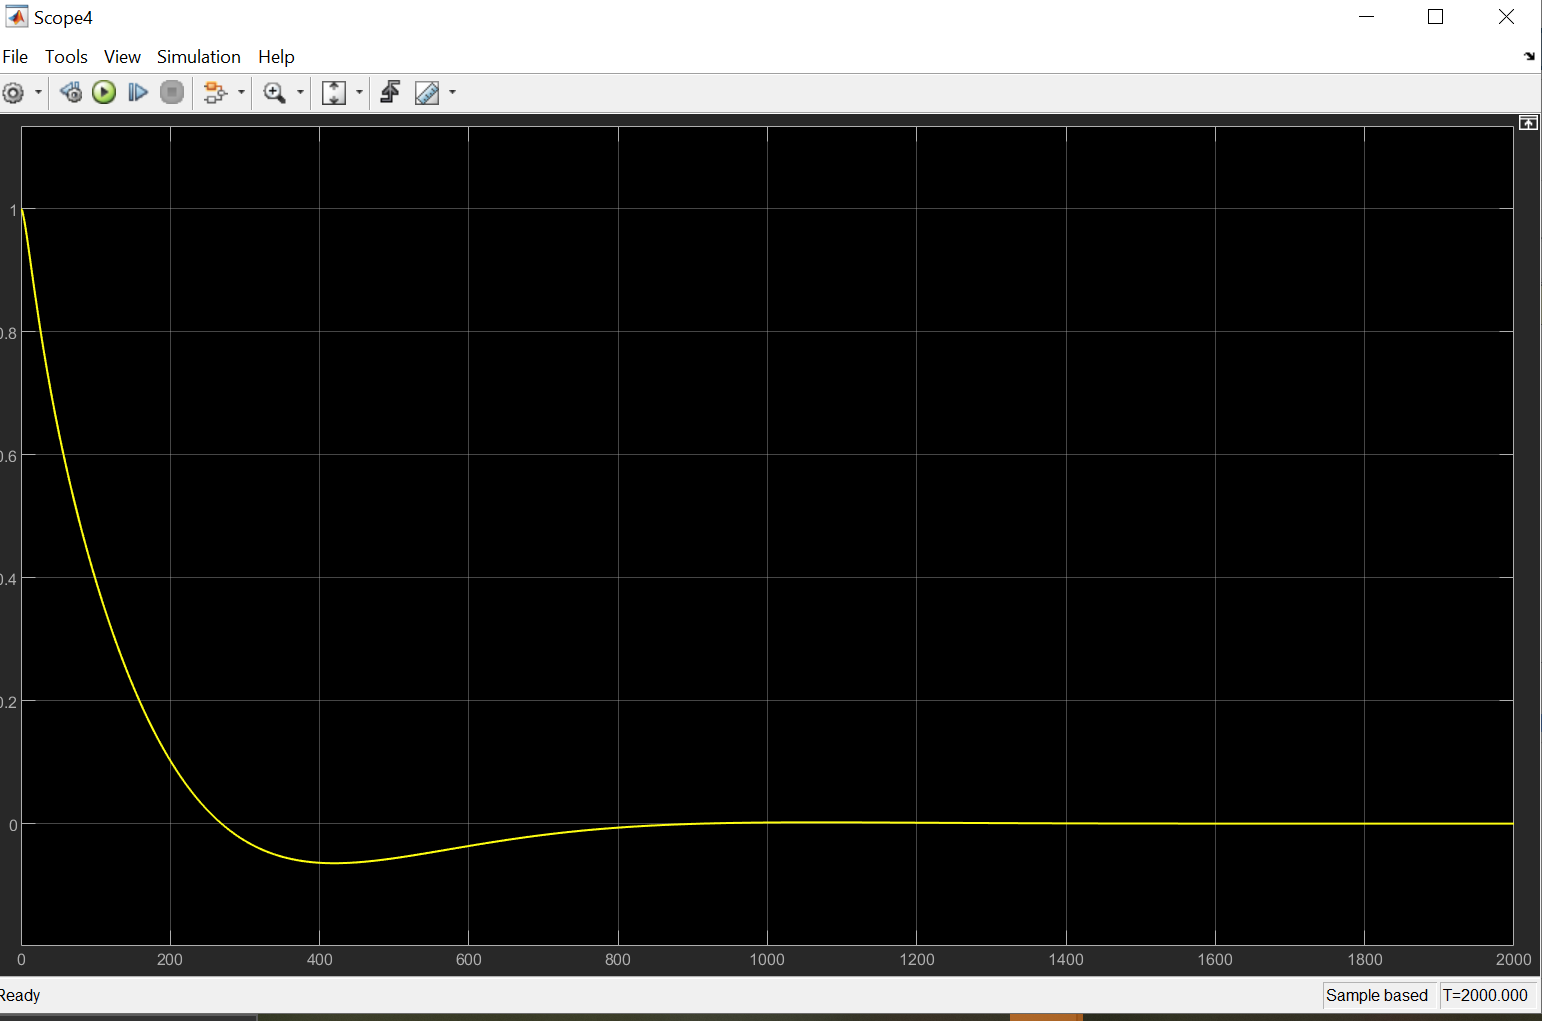
\includegraphics[scale=0.45]{images/SSE_AfterPID_Simulink.png}
	\caption{SSE Calculation after PID in Simulink}
	\label{fig:SSE_AfterPID_Simulink}
\end{figure}

\begin{figure}[h!]
	\centering
	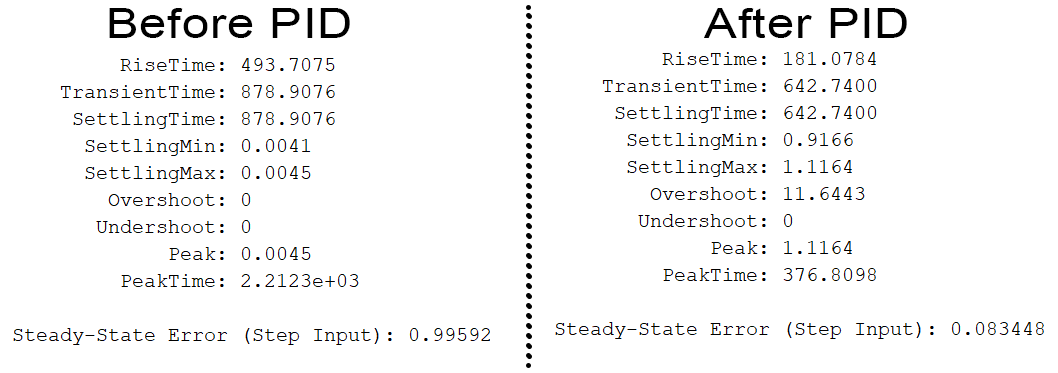
\includegraphics[scale=0.75]{images/SSE_MATLAB.png}
	\caption{SSE Calculation before and After PID in MATLAB}
	\label{fig:SSE_MATLAB}
\end{figure}

\subsection{SSE for Ramp Response}
This section describes the SSE computation before and after PID Design using Ramp Signal as input.

\subsubsection{SSE Calculation before PID Design}
The procedure is same as described in previous section \ref{SSE_StepResponseSec} but with Ramp as input signal. The sketch for computing SSE for Ramp is shown in Figure \ref{fig:SSE_Sketch_Ramp}.

\begin{figure}[h!]
	\centering
	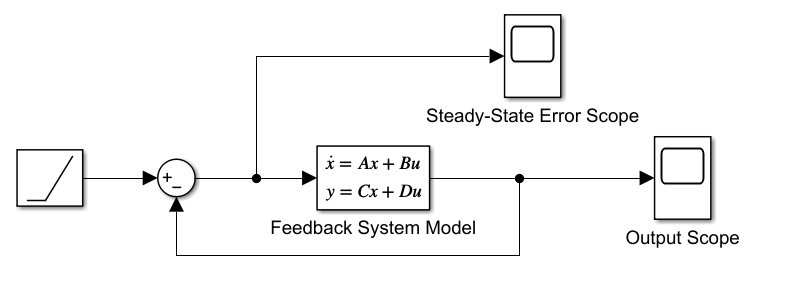
\includegraphics[scale=0.75]{images/SSE_Sketch_Ramp.png}
	\caption{Unity Feedback System With Ramp as Input}
	\label{fig:SSE_Sketch_Ramp}
\end{figure}

\begin{figure}[h!]
	\centering
	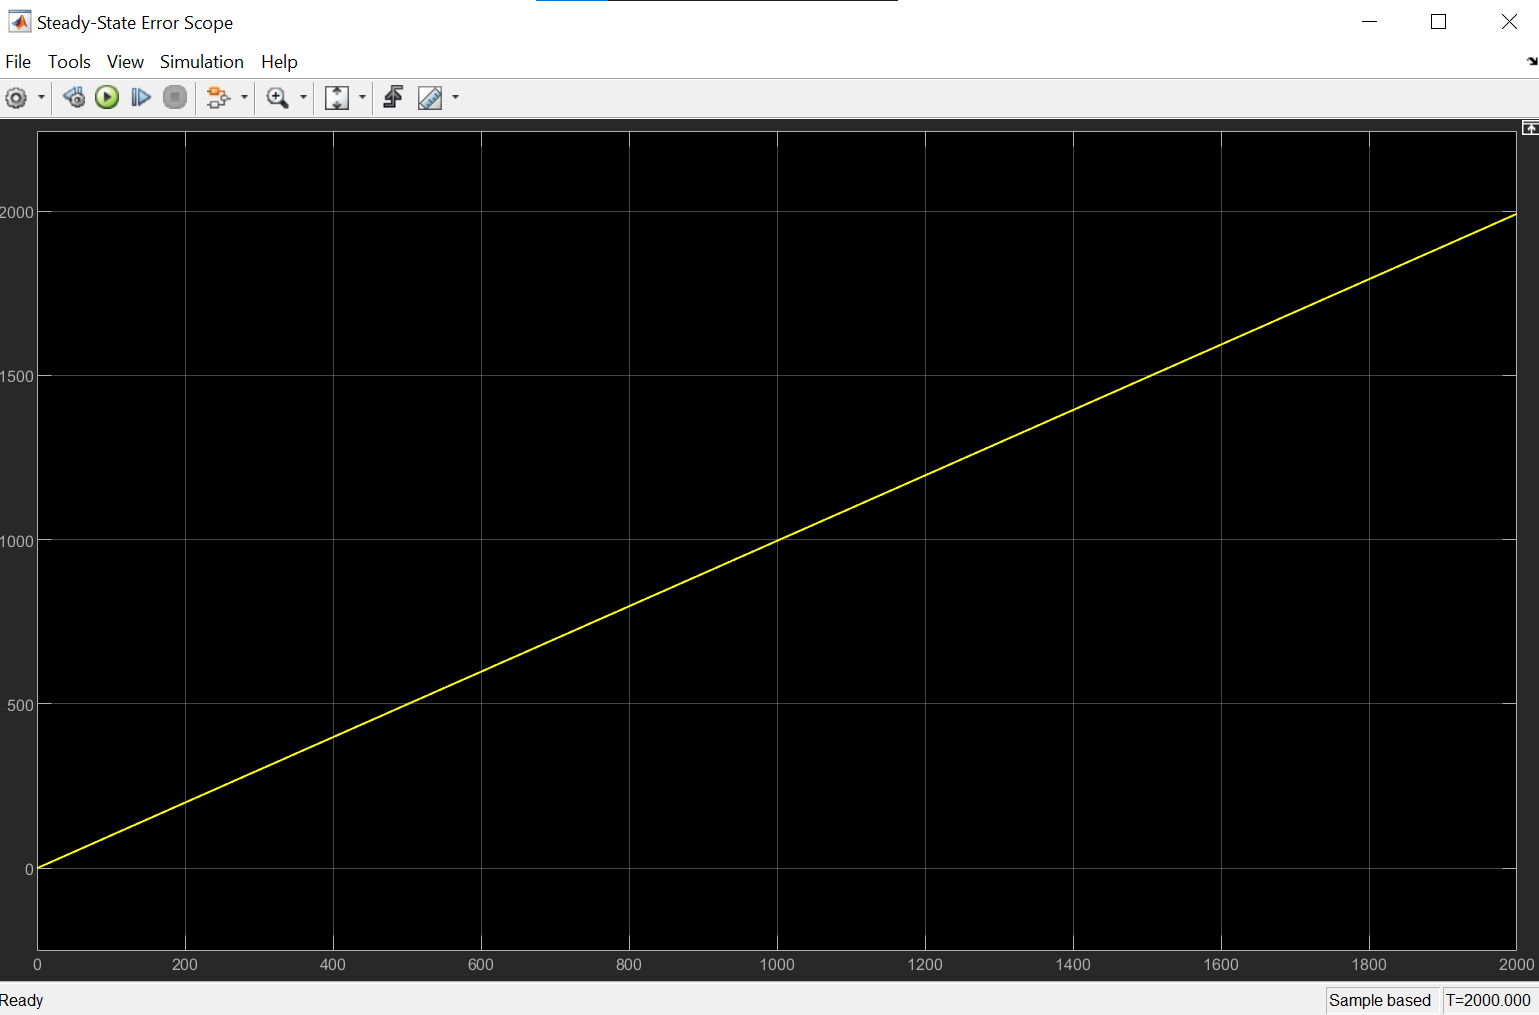
\includegraphics[scale=0.5]{images/SSE_BeforePID_Simulink_Ramp.png}
	\caption{SSE Calculation before PID in Simulink for Ramp}
	\label{fig:SSE_BeforePID_SimulinkRamp}
\end{figure}


\subsubsection{SSE Calculation after PID Design}
After connecting the PID Controller in series as shown in Figure \ref{fig:PIDController}, the SSE reaches almost to 75 and the response is still inifinite. The ramp response is shown in figure \ref{fig:rampResponse_PID_MATLAB} (MATLAB) and Figure \ref{fig:rampResponse_PID_Simulink} (Simulink). The SSE value from MATLAB is 57.5251 for Ramp Input. 

\begin{figure}[h!]
	\centering
	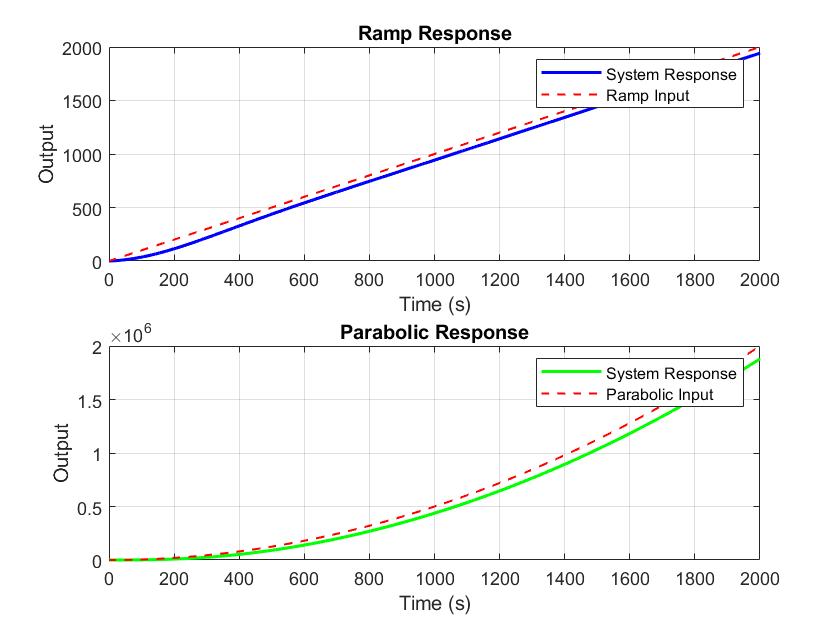
\includegraphics[scale=0.5]{images/rampparabolicResponse_PID_MATLAB.png}
	\caption{Ramp Response after PID in MATLAB}
	\label{fig:rampResponse_PID_MATLAB}
\end{figure}

\begin{figure}[h!]
	\centering
	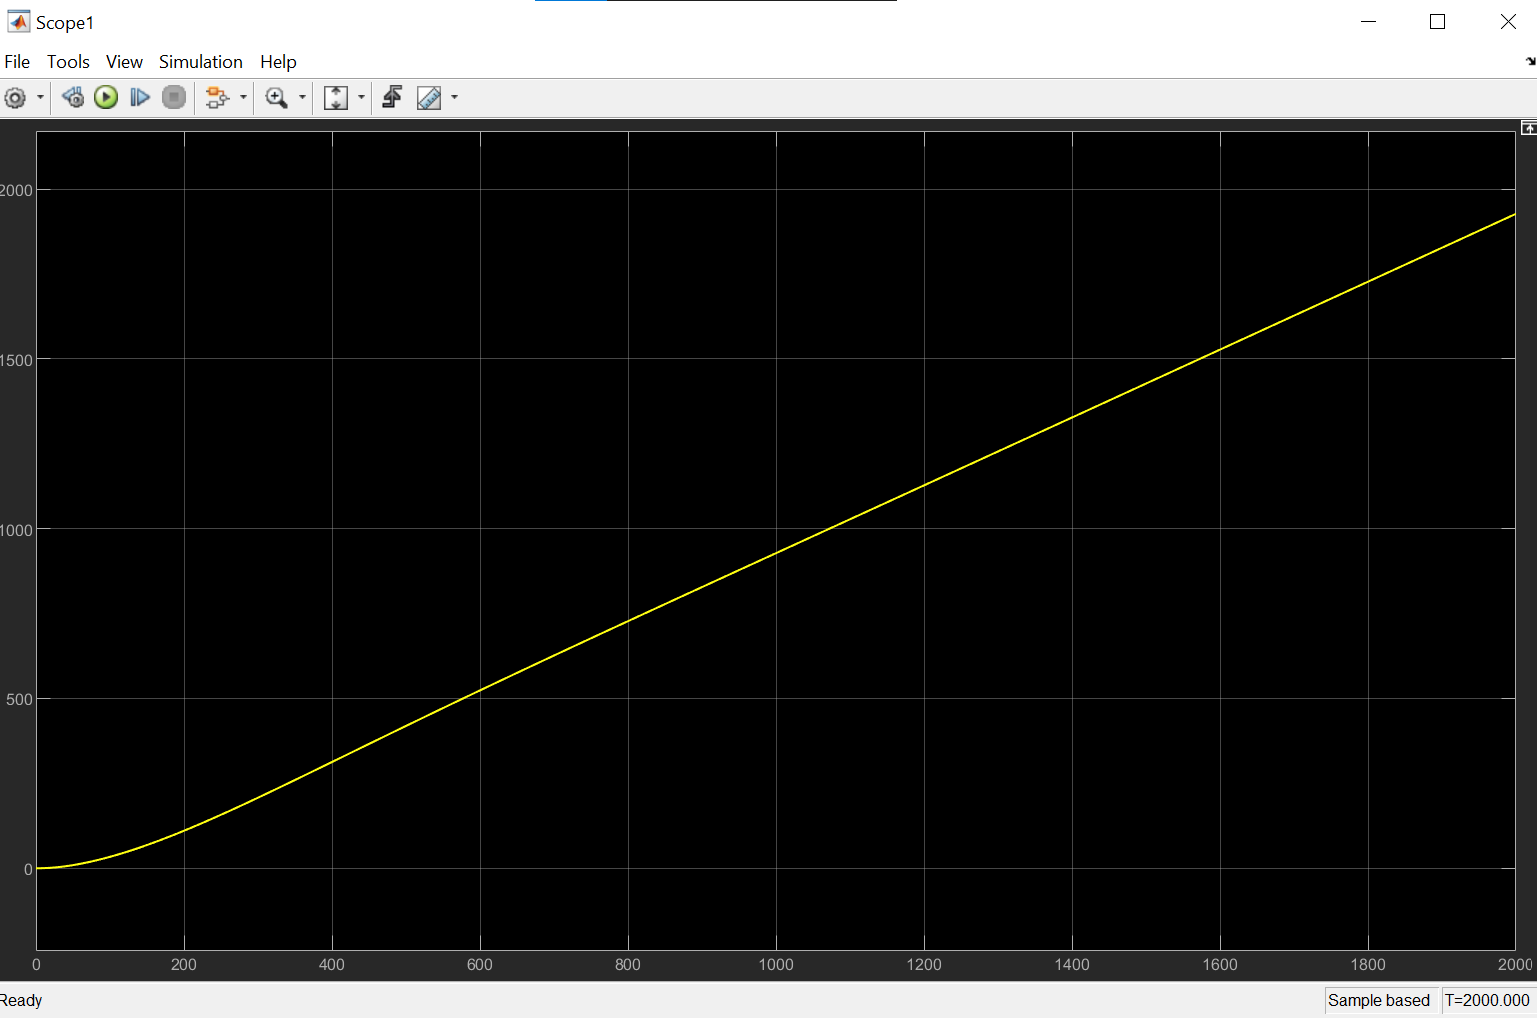
\includegraphics[scale=0.45]{images/rampResponse_PID_Simulink.png}
	\caption{Ramp Response after PID in Simulink}
	\label{fig:rampResponse_PID_Simulink}
\end{figure}

\subsection{SSE for Parabolic Response}
This section describes the SSE computation before and after PID Design using Parabolic Signal as input.

\subsubsection{SSE Calculation before PID Design}
The procedure is same as described in previous section \ref{SSE_StepResponseSec} but with Parabolic as input signal. The sketch for computing SSE for Parabolic is shown in Figure \ref{fig:SSE_Sketch_Parabolic}.

\begin{figure}[h!]
	\centering
	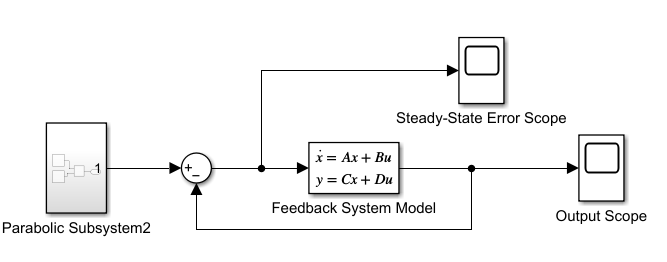
\includegraphics[scale=0.75]{images/SSE_Sketch_Parabolic.png}
	\caption{Unity Feedback System With Parabolic as Input}
	\label{fig:SSE_Sketch_Parabolic}
\end{figure}

\begin{figure}[h!]
	\centering
	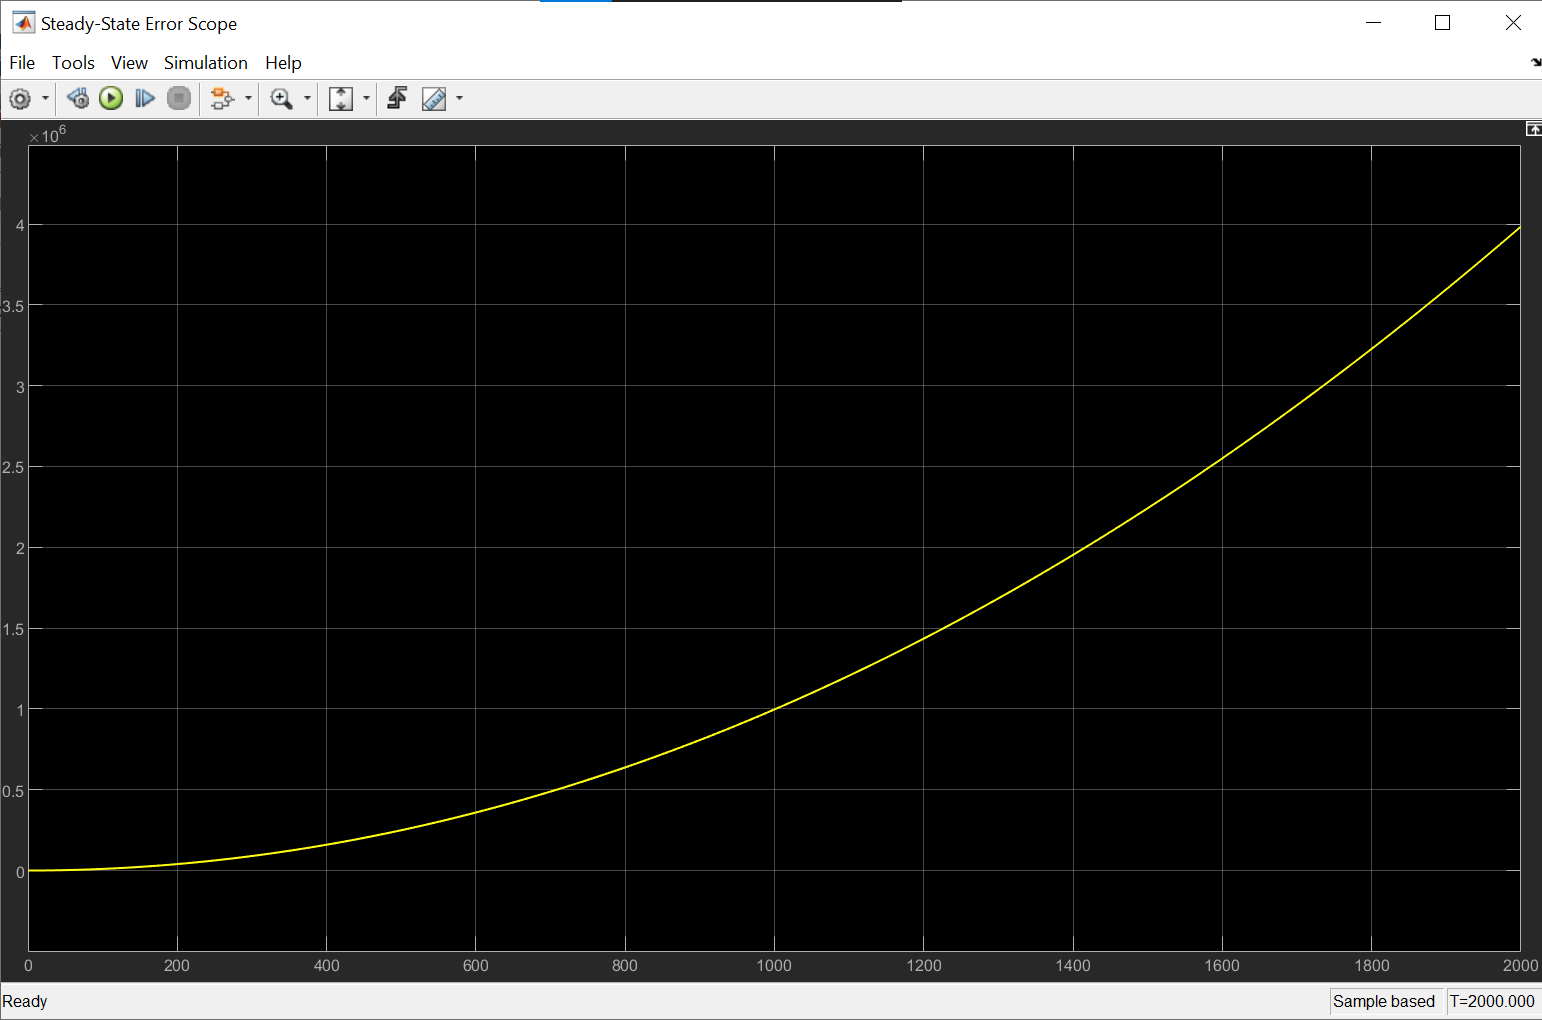
\includegraphics[scale=0.5]{images/SSE_BeforePID_Simulink_Parabolic.png}
	\caption{SSE Calculation before PID in Simulink for Parabolic}
	\label{fig:SSE_BeforePID_SimulinkParabolic}
\end{figure}


\subsubsection{SSE Calculation after PID Design}
After connecting the PID Controller in series as shown in Figure \ref{fig:PIDController}, the SSE reaches to infinity and the response is also inifinite. The Parabolic response is shown in figure \ref{fig:rampResponse_PID_MATLAB} (MATLAB) and Figure \ref{fig:parabolicResponse_PID_Simulink} (Simulink).

%\begin{figure}[h!]
%	\centering
%	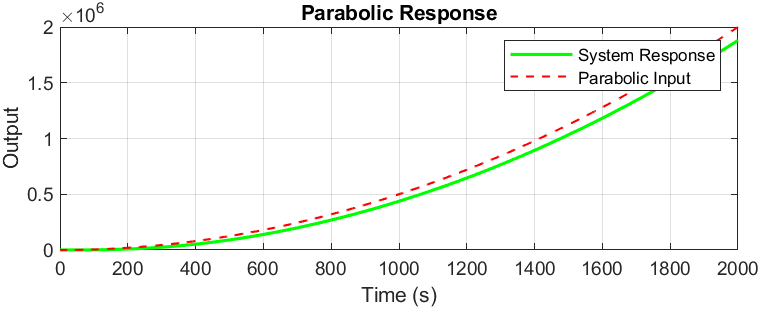
\includegraphics[scale=0.75]{images/parabolicResponse_PID_MATLAB.png}
%	\caption{Parabolic Response after PID in MATLAB}
%	\label{fig:parabolicResponse_PID_MATLAB}
%\end{figure}

\begin{figure}[h!]
	\centering
	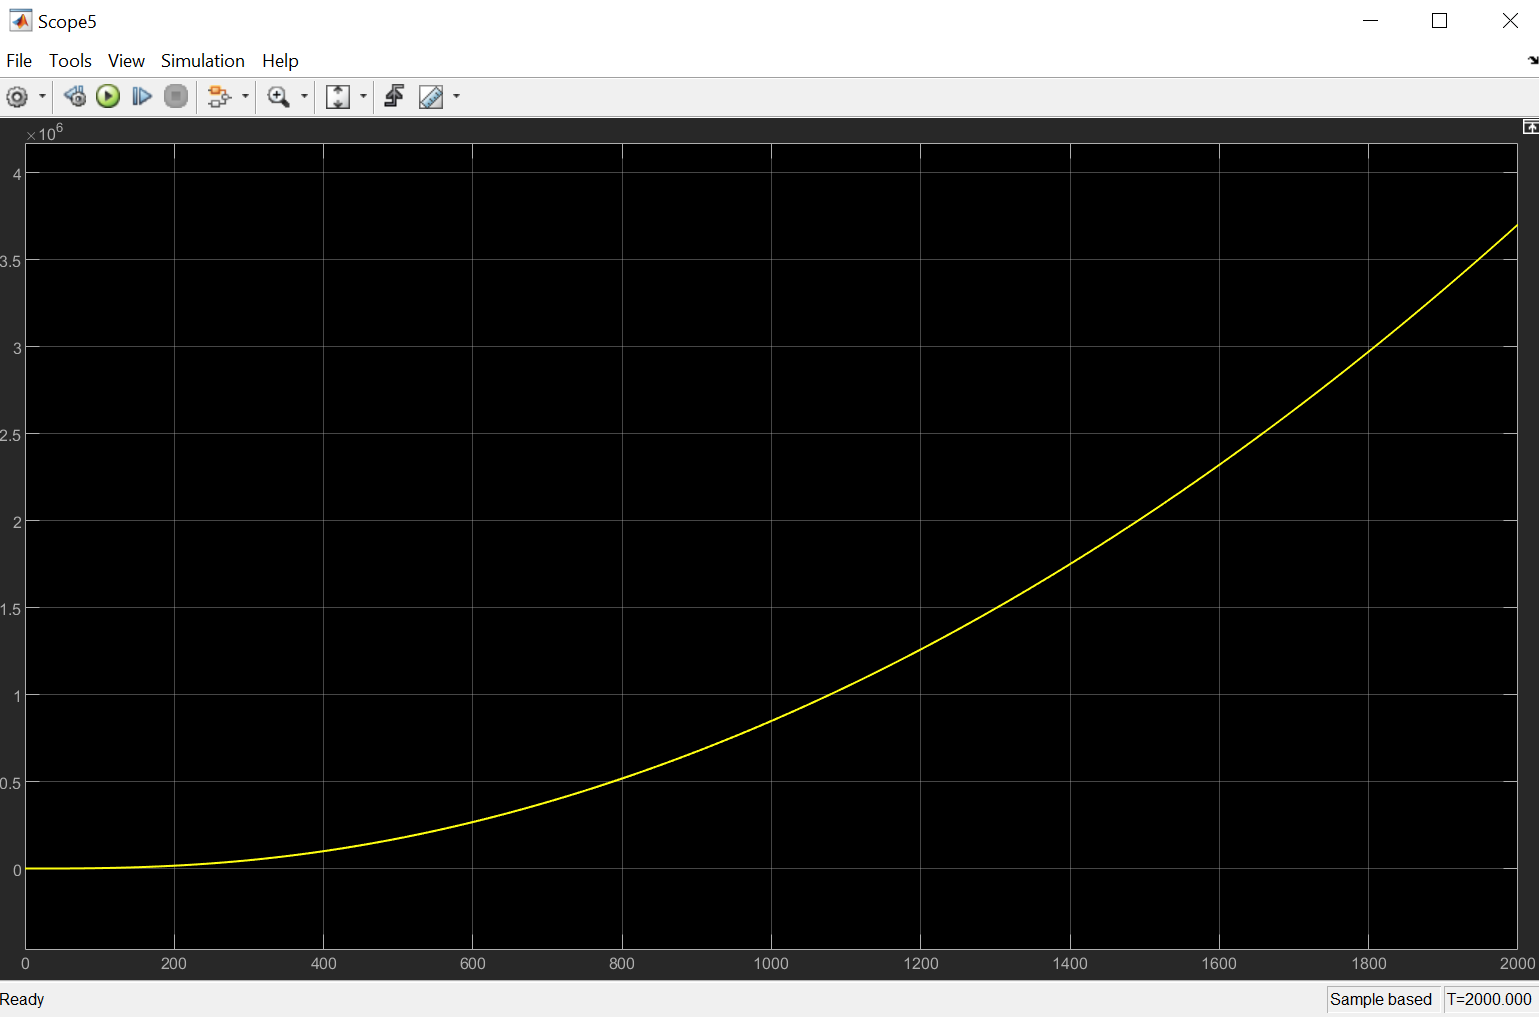
\includegraphics[scale=0.45]{images/parabolicResponse_PID_Simulink.png}
	\caption{Parabolic Response after PID in Simulink}
	\label{fig:parabolicResponse_PID_Simulink}
\end{figure}


\vskip400pt
\section{Conclusion}
In this project, we analyzed and designed a control system for a state-space model derived from Problem 22 in the Norman Nise book. The system stability was verified using eigenvalues, poles, and step response analysis, confirming that the system is inherently stable. Simulation results for the PID controller offered a significant reduction in steady-state error while maintaining acceptable transient behavior. 
This project highlights the importance of system analysis and appropriate controller design in achieving optimal performance for control systems.
  
\end{document} 